
%%%%%%%%%%%%%%%%%%%%%%%%%%
\chapter{Materials and Methods}
\label{ch:3methods}


Following a line of recent works \shortcites{karoly2017circadian, baud2018multi}\cite{karoly2017circadian, baud2018multi, baud2020chance}, we consider a probabilistic approach to seizure prediction, expressed via an algorithm we term Bayesian Seizure Likelihood Estimation (BSLE)\footnote{code can be found at \url{https://github.com/noamsgl/msc} under the MIT license.}.

%%%%%%%%%%%%%%%%%%%%%%%%%%%%%%%%%%%%%%%%%%%%%%%%%%%%%%%%%%%%%%%%%%%%%%%%%%%%%%%%%%%%%%%%%%%%%%%%%%%%%%%%

\section{Data}
In this work we use the \emph{Canine-Epilepsy Dataset} \shortcites{davis2011novel}\cite{davis2011novel, kaggle2014contests}. Three dogs with naturally occurring epilepsy are monitored continuously, for 330/451/475 days for Dog 1, Dog 2, and Dog 3, respectively. The monitoring systems consist of 16-electrode EEG sensors implanted in each brain, digitally sampling at the rate of 400 Hz. In addition, a sequence of timestamps are provided for each dog, marking the observed seizure events (\aka annotations).

\NS[inline]{insert illustration of data collection}


\subsection{Train-test split}
\NS[inline]{write about train-test split (offline-online modes)}
%For the competition, the dataset was split into segments of length 1 second, each labeled as interictal or ictal. The training set is composed of 178 ictal and 418 interictal segments, which is relatively balanced compared to the high imbalance found in reality.

\section{Probabilistic model}
We capture the notion of EEG observations and seizure events by random variables (r.v.s):

\begin{align}
	 e_t \sim E(t) &\in \Omega_E = \mathbb{R}^{c \times \tau}\\
	 s_t \sim S(t) &\in \Omega_S = \{0, 1\}
\end{align}

where $\Omega_{E/S}$ is the sample space for each variable $E$ and $S$, respectively. $c$ is the number of EEG-channels, $\tau$ is the duration of EEG recorded (\aka segment length). We define the event that a seizure occurred at time $t$ as $\{S(t) = 1\}$.

Our work introduces a multilevel probabilistic model for dataset annotations (see figure \ref{fig:3methods:bsle_net}). The model is inspired by the hypothesis that clinical annotations are very precise but not highly sensitive. That is, we believe that a proportion of seizures don't become recorded annotations, and explicitly take this belief into account in our model. These can often be explained by the annotator's reliance on video-footage and a possible lack of clinical symptom manifestations\NS{add citation}.

% Full Bayesian Seizure Annotation Model
\begin{figure}[H]

  \tikz{

    % nodes
     \node[obs] (e) {$e_{t}$};%
     \node[latent, above=of e, xshift=1cm] (s) {$s_{t}$}; %
     \factor[above=of s, yshift=0.75cm] {cox} {right:Cox$(\lambda_{\phi_i})$} {} {}; 
     
    \node[latent, left=of cox] (phi) {$\phi_i$};
    \node[obs, below=of s, xshift=1cm] (a) {$a_{t}$};%
    \node[latent, below=of a] (o) {$o_{t}$}; %
    \factor[left=of o, xshift=-1cm] {ber} {above:Ber$(p)$} {} {};
    
    % gates
    \gate[] {seen} {(a)} {o};
    
    % edges
     \edge {s} {e, a}
     \edge {ber} {o}
    %  \edge {o} {a}
     \edge {cox} {s}
     \edge {phi} {cox}
    
    % plates
    
    \plate[inner sep=10pt] {plate1} {(e)(a)(s)(ber)(o)} {time $t$}; %
    \plate[inner sep=10pt] {plate2} {(plate1)(cox)(phi)} {subject $i$}; %

    % text
     \node[text width=6cm, anchor=west, right] at (4,1)
     {
       \begin{alignat*}{3}
        \phi_i & \sim \mathcal{D}_{\phi_i} \quad && \text{// subject-specific params}\\
        \lambda & _{\phi_i} (t) \gets \text{prior}_{\phi_i} : \Rplus \to \Rplus \quad &&\text{// intensity function}\\
        s_t & \sim \text{Cox}(\lambda_{\phi_i}) && \text{// stochastic counting process}\\
        e_t & \mid s_t \sim \mathcal{D}_{E \mid S} && \text{// EEG conditioned on seizure var}\\
        o_t & \sim \text{Bernoulli}(p) && \text{// was the seizure observed?}\\
        a_t & \sim s_t \text{ if } o_t \text{ else } 0 && \text{// sample annotation}\\
       \end{alignat*}
     };
   }
 \Caption{Probabilistically Modeling Seizure Occurrence, EEG signal and Annotations across Time and Subjects}{The nodes represent random variables. The shaded nodes $e$ and $a$ represent the observed variables EEG and Annotations, respectively. The rest are latent variables, which can be inferred with Bayes' theorem. The plates represent levels of hierarchy along which the model is replicated, such as time or subject, and the arrows indicate causal direction.}
  \label{fig:c3bsle:bsle_net}
\end{figure}

The model describes the process by which seizure annotations are generated. The $W, k$ parameters control the shape of the individual's circadian profile. $\lambda(t)$ is the latent intensity function for the seizure-occurrence Cox process. After sampling a seizure-history $S(t)$, each seizure is dropped with a probability of $p$, and becomes an observable annotation with probability $1-p$. This reflects annotators' missing sections of the EEG recordings, as well as sub-clinical seizures.

More formally (see algorithm \ref{alg:ann_model}), the probability of obtaining an annotation at time $t$ is a zero-inflated seizure occurrence model. Sequentially, the seizure-occurrence model is a Cox process with a stochastic intensity function $\lambda(t)$. In turn, the intensity function $\lambda(t)$ is a mixture model of 24 von-Mises distributions, one for each hour of the day. Finally, the weights $W$ and common spread $k$ parameters assume noninformative priors.


% \begin{definition}[von Mises Distribution]
% The von Mises probability density function for the angle $x$ is given by $f_{v.M.}(x; \mu, k) = \frac{\exp{k \cos (t - \mu)}}{2 \pi I_0(k)}$.
% \end{definition}

\begin{algorithm}
\caption{Seizure Annotation Model}
\label{alg:ann_model}
\begin{algorithmic}
\State $k \sim Exp(1)$
\State $\alpha[0,...,23] \gets 1$
\State $W[0,...,23] \sim Dir(\alpha)$
\State $\lambda(t) \gets \sum_{i=0}^{23} W[i] \cdot f_{v.M.}(t; i, k)$
\State $S(t) \sim Cox(\lambda)$
\State $Annotation(t) = ZeroInflated(S(t), p)$
\end{algorithmic}
\end{algorithm}
\NS[inline]{revise algorithm}
% https://tex.stackexchange.com/a/460920

\section{Bayesian Seizure Likelihood Estimation}
\NS[inline]{rewrite BSLE section}

In the case of epilepsy, handling uncertainty in the face of evidence plays a major role, thus naturally appealing to the mathematical machinery termed Bayes' theorem\footnote{much credit is due to Pierre Simon Laplace, who developed the form in common use today \cite{mcgrayne2011theory}.}.

We apply Bayes' theorem to estimate the updated likelihood of a seizure after observing an EEG signal:

\begin{align}
    \underset{posterior}{\prob(S \mid E)} = \frac{\prob(E \mid S) \prob(S)}{\prob(E)} \propto \underset{likelihood}{\prob(E \mid S)} \cdot \underset{prior}{\prob(S)}
\end{align}

We now introduce our method to calculate the likelihood and prior, thus completing the description of our inference procedure. In the next chapters we will show experimental results and discuss pros and cons of this method.

\begin{align}
    \prob(S \mid E) = 1 - \frac{\prob(\neg S) \prob(E \mid \neg S)}{\prob (E)}
\end{align}

due to the assumption $\prob(S) + \prob(\neg S) = 1$.

\begin{align}
    \prob(E \mid \neg S) = \prob(\{\hat p (e \mid \theta^*) \leq \hat p(E \mid \theta^*)\})
\end{align}

\begin{align}
    \prob(E) = \prob(\{pdf(e) \leq pdf(E)\})
\end{align}
\subsection{BSLE - likelihood}

\subsubsection{EEG embedding}
Representing a typical 10-second EEG segment requires about \num{6.4e4} scalar values in it's raw form, thus special care is taken to overcome the curse of dimensionality. In this work, we embed the EEG data in a low-dimensional space, namely the space of GP parameters. We found the ictal embeddings to be distinguishable from the interictal embeddings even after the dimensionality reduction.

Following the described embedding of the EEG signal in the space of GP parameters, we adopt the new notation $\EEGt{} \in \mathbb{R}^d$, where the new dimension satisfies $d \ll d' \times T$.

\subsubsection{Gaussian process parameters embedding}
Inference of Gaussian process (GP) parameters is a well-documented approach to modeling time-series data \cite{rasmussen2003gaussian}. The extension to multitask GPs enables modeling of multivariate time-series, such as the case of multi-lead EEG signals.

\begin{figure}[htbp]
    \centering
    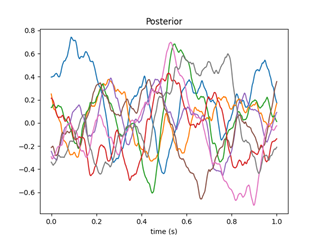
\includegraphics[width=0.4\floatwidth]{3Methods/Figs/GP/posterior_draws.png}
    \Caption{Embedding EEG with GP hyperparameters}{
	Posterior draws from a Gaussian process fit to maximize the likelihood of an observed single-channel EEG segment.
	\protect \NS[inline]{replace with vectorized image}
	\protect \NS[inline]{add original sample}
    }
    \label{fig:3methods:posterior_draws}
\end{figure}


For each EEG segment $x$, the preprocessing steps include:

\begin{enumerate}[label=\roman*]
    \item Normalizing $x$ by subtracting the mean and dividing by the standard deviation of the training set.
    \item initializing a GP model with zero mean, a scaled Matérn-1.5 kernel, and a rank-1 multitask covariance kernel.
    \item Optimizing the model's parameters to obtain a maximal marginal log-likelihood (details in appx. \ref{apx:GPTraining}).
\end{enumerate}

The optimized model's parameters $\theta$ are persisted and used henceforth to represent the original EEG segment $x$.


\subsubsection{$\mathcal{Z}(E)$ - Novelty Score}
\NS[inline]{reconsider if novelty score is necessary}
%The model for normal EEG was developed using the interictal embeddings of dimensions $\Vec{\theta} \in \mathbb{R}^2$ in the single-channel case or$\Vec{\theta} \in \mathbb{R}^5$ in the double channel case. A Gaussian mixture model with 2 components was fit with the expectation-maximization algorithm to the interictal embeddings since these represent the normal (non-seizure) EEGs. The fitted model approximates the probability distribution of the EEG data represented in the parameter space, conditioned on the previously seen data, $\hat p (\Vec{\theta} \mid \{ \Vec{\theta_i} \})$.
%Finally, for a given EEG clip represented by the GP parameters as $\Vec{\theta}^{new}$, we define the novelty score by:
%
%\begin{align}
%    z(\Vec{\theta}^{new}) = - \log \hat p (\Vec{\theta} \mid \{ \Vec{\theta_i} \})
%\end{align}
%


%\begin{align}
%    p_{value}(\Vec{\theta} ^{new}) = \mathbf{Pr} (\mathbb{I}_{ictal} \mid \Vec{\theta}^{new}) = \frac{|\{ \Vec{\theta}_i \mid z(\Vec{\theta}_i) \ge z(\Vec{\theta}^{new})\}|}{\{ \Vec{\theta_i}\}}
%\end{align}

%Thus, the tail-area probability $p_{value}(\Vec{\theta} ^{new})$ function maps data samples to the interval $[0, 1]$, such that more anomalous samples are given smaller p-values.

%For normal EEG data, the new observation $\Vec{\theta}^{new}$ will be similar to previously seen normal observations in $\{ \Vec{\theta_i} \}$, therefore the likelihood will be high. Consequently, the negative log likelihood will be low and so the novelty score will be low. Conversely, for abnormal (seizure) data, the data will be dissimilar, and the likelihood will be low, and so consequently the novelty score $z(\Vec{\theta}^{new})$ will be high.


We derive a \emph{generative} novelty score $\mathcal{Z}(E)$ as a substitute for the likelihood, $P(E \mid S) \propto \mathcal{Z}(E)$.


For a patient with epilepsy, we hypothesize that the anomalies in EEG data are inherently likely to reflect seizures. Thus, we substitute the likelihood term in Bayes' theorem with the novelty score $z(\theta)$ to provide an estimate of the likelihood of observing an EEG:

\begin{align}
    P(E \mid S) \equiv z(E)
\end{align}

\subsection{BSLE - Prior}

\subsubsection{Circadian distribution prior}
The \emph{Circadian distribution prior} is the same one used by \shortcites{karoly2017circadian}\citet{karoly2017circadian}, based on a mixture of von Mises distributions (see equation \ref{eq:2background:vm_density}).

Our work complements the current understanding of the prior's contribution to predictive performance, and has many features that distinguish it from prior work.
\NS[inline]{list of ways this work differs from prior works}


\section{Configuring seizure alerts}

Based on the posterior class probability $\prob(S \mid E, t)$, we will configure warning alerts:
\NS[inline]{determine method to configure alerts (metric-dependent?)}

